\documentclass{standalone}

\usepackage{tikz}

\begin{document}

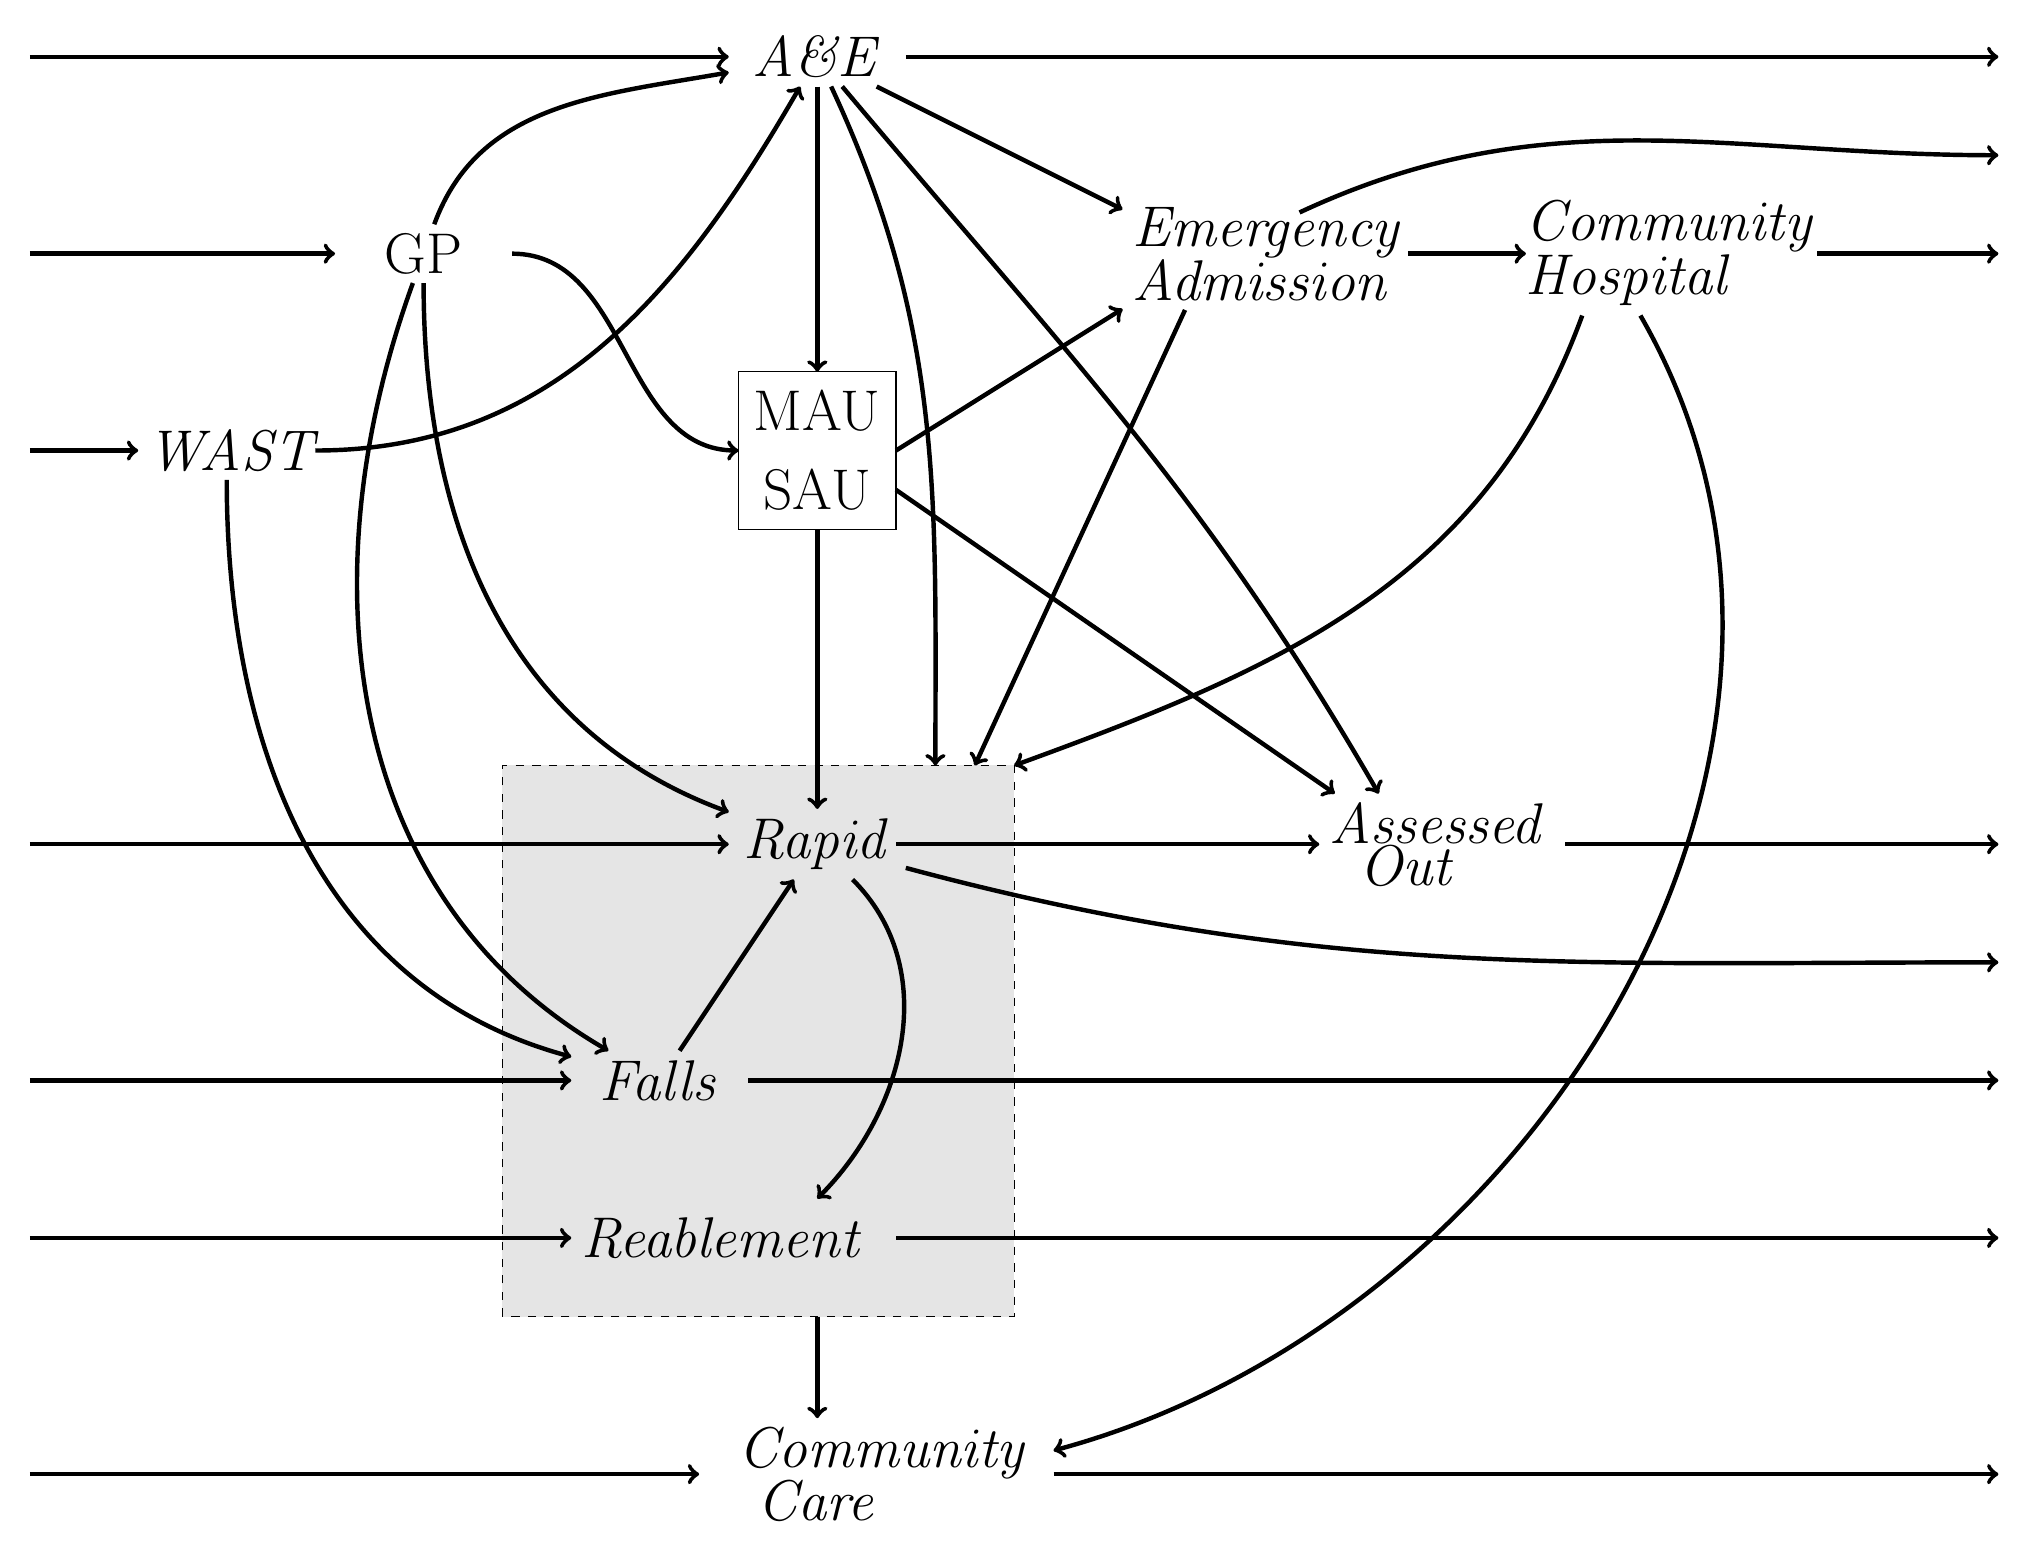
\begin{tikzpicture}


\draw[draw=black, fill=none] (9, 9) rectangle (11, 11);
\draw[draw=black, fill=gray!20, dashed] (6, -1) rectangle (12.5, 6);

\node[text width=2cm, align=center] (GP) at (5, 12.5) {\huge{GP}};
\node[text width=2cm, align=center] (AE) at (10, 15) {\huge{\textit{A\&E}}};
\node[text width=2cm, align=center] (MS) at (10, 10.5) {\huge{MAU}};
\node[text width=2cm, align=center] (MS) at (10, 9.5) {\huge{SAU}};
\node[text width=2cm, align=center] (RPD) at (10, 5) {\huge{\textit{Rapid}}};
\node[text width=2cm, align=center] (EM) at (15, 12.5) {\huge{\textit{Emergency\\Admission}}};
\node[text width=2cm, align=center] (CH) at (20, 12.5) {\huge{\textit{Community\\Hospital}}};
\node[text width=2cm, align=center] (AO) at (17.5, 5) {\huge{\textit{Assessed\\Out}}};
\node[text width=2cm, align=center] (FLS) at (8, 2) {\huge{\textit{Falls}}};
\node[text width=2cm, align=center] (RBL) at (8, 0) {\huge{\textit{Reablement}}};
\node[text width=2cm, align=center] (CC) at (10, -3) {\huge{\textit{Community\\Care}}};
\node[text width=2cm, align=center] (WAST) at (2.5, 10) {\huge{\textit{WAST}}};

\draw[ultra thick, ->] (GP) edge[out=70, in=-170] (AE);
\draw[ultra thick, ->] (GP) edge[out=-90, in=160] (RPD);
\draw[ultra thick, ->] (AE) -- (EM);
\draw[ultra thick, ->] (AE) edge[out=-50, in=120] (AO);
\draw[ultra thick, ->] (11, 5) -- (AO);
\draw[ultra thick, ->] (GP) edge[out=0, in=180] (9, 10);
\draw[ultra thick, ->] (AE) -- (10, 11);
\draw[ultra thick, ->] (10, 9) -- (RPD);
\draw[ultra thick, ->] (11, 9.5) -- (AO);
\draw[ultra thick, ->] (11, 10) -- (EM);
\draw[ultra thick, ->] (AE) edge[out=-65, in=90] (11.5, 6);
\draw[ultra thick, ->] (0, 12.5) -- (GP);
\draw[ultra thick, ->] (0, 5) -- (RPD);
\draw[ultra thick, ->] (17.5, 12.5) -- (19, 12.5);
\draw[ultra thick, ->] (19.5, 5) -- (25, 5);
\draw[ultra thick, ->] (0, -3) -- (8.5, -3);
\draw[ultra thick, ->] (13, -3) -- (25, -3);
\draw[ultra thick, ->] (0, 0) -- (RBL);
\draw[ultra thick, ->] (0, 2) -- (FLS);
\draw[ultra thick, ->] (GP) edge[out=-110, in=150] (FLS);
\draw[ultra thick, ->] (CH) edge[out=-110, in=20] (12.5, 6);
\draw[ultra thick, ->] (EM) -- (12, 6);
\draw[ultra thick, ->] (RPD) edge[out=-45, in=45] (10, 0.5);
\draw[ultra thick, ->] (FLS) -- (25, 2);
\draw[ultra thick, ->] (RPD) edge[out=-15, in=180] (25, 3.5);
\draw[ultra thick, ->] (11, 0) -- (25, 0);
\draw[ultra thick, ->] (22.7, 12.5) -- (25, 12.5);
\draw[ultra thick, ->] (0, 10) -- (WAST);
\draw[ultra thick, ->] (WAST) edge[out=-90, in=165] (FLS);
\draw[ultra thick, ->] (WAST) edge[out=0, in=-120] (AE);
\draw[ultra thick, ->] (10, -1) -- (CC);
\draw[ultra thick, ->] (FLS) -- (RPD);
\draw[ultra thick, ->] (0, 15) -- (AE);
\draw[ultra thick, ->] (AE) -- (25, 15);
\draw[ultra thick, ->] (EM) edge[out=25, in=-180] (25, 13.75);
\draw[ultra thick, ->] (CH) edge[out=-60, in=15] (13, -2.7);




\end{tikzpicture}

\end{document}
